\chapter{Related Work}
\label{ch:related-work}

\todo{introduce in related work, differentiate the importance of datasets}
Describe relevant scientific literature related to your work.

%%%%%%%%%%%%%%%%%%%%%%%%%%%%%%%%%%%%%%%%%%%%%%%%%%%%%%%%%%%%%%%%%%%%%%%%%%%%%%%%

\section{Datasets of UI Trees}
\label{sec:datasets-of-ui-trees}

A fundamental part of training \gls{ann}s are solid and large datasets, which provide enough information to gain the expected result.
Therefore, these datasets have to fulfill some requirements, like completeness, quantity, feature richness, topicality and (public) accessibility.
In the follows, papers of thematic relevance are verified on the basis of these criteria.

\subsection{ERICA}
\label{subsec:erica}

ERICA is a design and interaction mining application, which allows gathering \ti{interaction traces} by capturing the users activity on Android apps~\cite{deka2016erica}.
This is accomplished through a web-based interaction layer in contrast to the other common approach of using \ti{accessibility services} directly.
They justify that approach by the lack of need to install additional applications, as only a browser is required.
A further reason is the response latency of the commonly used \ti{UiAutomator}, which cannot collect the data in time.
Also they argue that capturing and simultaneously interacting with the apps may overload the user device and challenges the user experience.
Therefore the much more powerful servers take the task of capturing the UI trees.
The apps are hosted on multiple physical devices with a modified Android OS directly connected with the server.
ERICA captures UI screens and user flows by tracking UI changes.
They then used this data to form k-mean clusters from the UI elements (visual and textual features) and the interactive elements (icons and buttons).
Based on the clusters they then build classifiers and trained an AutoEncoder (\ref{subsec:autoencoder}) to determine the flows from the test dataset.
The authors worked out 23 common user flows (from over a thousand popular Android apps) which aim to provide complementary, promising or new design patterns and trends.

%- data-driven app design application
%- gathers user interaction trace > 1000 popular apps
%- 3000 flow examples

%\todo{descibe how they worked out the 23 user flows, which Autoencoder they used etc.}

%which employs a human-powered approach over an automated one:
%- More realistic results
%- required user input, which cannot emulated, Google Captcha, real data
%- humans detect the completion of UI updates \cite{deka2016erica}
%- erica is quite outdated

\subsection{Rico / RicoSCA}
\label{subsec:rico}

Rico~\cite{deka2017rico} is the successor of ERICA.
It aims to help perform better at designing and support the creation of adaptive UIs.
As far as known to date this is the largest collection of mobile app designs and traces with covering 72k UI screens in 9.7k Android apps.
Like its predecessor Rico uses a web-based approach to collect user traces.
It enables the applications like searching for designs, generation of UI layouts and code, modeling of user interactions, and prediction of user perception.
It exposes visual, textual, structural, and interactive design properties of more than 72k unique UI screens.
Unfortunately the dataset doesn't include interaction traces for app to app transitions or interactions with the Android OS itself.
In table~\ref{tab:rico_view_hierarchy_attributes} a collection of all view hierarchy attributes is shown with their meaning.
These were extracted by iterating over all view hierarchy files contained in the traces of the dataset.
This gives insights in what attributes were recorded in the Rico dataset and what relevance they may have during training the model.
The authors of Rico used their dataset to train a 64-dimensional UI layout vector~\ref{subsec:embedding} with an AutoEncoder \ref{subsec:autoencoder}.
For their input they converted the UI layout hierarchy to an image with colored bounding boxes differentiating images and text.
This has the advantage to be able to deal with the high dimensions inside the UI tree.
But the conversion also most likely discards lots of meaningful information hidden in the UI tree semantics.

\begin{table}[htbp!]
  \small
  \centering
  \begin{tabular}{|l|c|c|>{\RaggedRight}p{0.5\linewidth}|}
    \hline
    \tb{Key} & \textbf{Type} & \textbf{Shape} & \textbf{Description} \\
    \hline
    \multicolumn{4}{c}{Per View} \\
    \hline
% Annotated by word2vec
%    \_is\_leaf\_node & bool & (1) & \\
%    \_caption\_preorder\_id & bool & (1) & \\
%    \_caption\_depth & bool & (1) & \\
%    \_caption\_node\_id & bool & (1) & \\
%    \_caption\_postorder\_id & bool & (1) & \\
    activity\_name & string & (1) & Name of the activity: e.g. \quotes{com.my\_app.AppName.MainActivity} \\
%    added\_fragments & [] & (None) & \\
%    active\_fragments & [] & (None) & \\
    is\_keyboard\_deployed & bool & (1) & Indicates if the keyboard is shown \\
    request\_id & int & (1) & Id used by the crawler to request the view \\
    \hline
    \multicolumn{4}{c}{Per Node} \\
    \hline
    abs-pos & bool & (1) & Indicates if position in \ti{bounds} is relative or absolute; if \ti{true}, \ti{rel-bounds} is set \\
    adapter-view & bool & (1) & Indicates that children are loaded via an adapter, see~\cite{android_adapterview} \\
    ancestors & [string] & (None) & Ancestors of current node, e.g. \quotes{android.view.View} \\
    bounds & [integer] & (4) & Absolute or relative boundaries, dependent on \ti{abs-pos} \\
    children & [node] & (None) & Child nodes \\
    class & string & (1) & \quotes{com.my\_app.lib.ui.views.DropDownSpinner} \\
    clickable & bool & (1) & User can interact by press / click \\
    content-desc & string & (1) & (Accessibility) description of the node \quotes{Interstitial close button} \\
    draw & bool & (1) & Indicates if this node is drawn on the canvas \\
    enabled & bool & (1) & Indicates if this node is in the enabled state \\
    focusable & bool & (1) & Indicates if this node can be focused \\
    focused & bool & (1) & Indicates if this node can is currently in focus \\
    font-family & string & (1) & States the font family, e.g. \quotes{sans-serif} \\
    long-clickable & bool & (1) & Indicates if this node has a long press action \\
    package & string & (1) & States which packages the node belongs to \quotes{com.my\_app.mypackage} \\
%    pointer & string & (1) & \todo{Presumably the saving address in the memory, e.g. \quotes{92690f4}} \\
    pressed & bool & (1) & Indicates if this node can is currently pressed \\
    rel-bounds & [integer] & (4) & Relative boundaries, if \ti{abs-pos} is set to \ti{true} \\
    resource-id & string & (1) & The unique resource identifier for this view \quotes{android:id/navigationBarBackground} \\
    scrollable-horizontal & bool & (1) & Indicates if this node can be scrolled horizontally \\
    scrollable-vertical & bool & (1) & Indicates if this node can be scrolled vertically \\
    selected & bool & (1) & Indicates if this node can is currently selected \\
    text & string & (1) & Text value if this node is a textual element \\
    text-hint & bool & (1) & Explanation text for text boxes or icons \\
    visibility & string & (1) & Indicates if this node is hidden, e.g. \quotes{visible}, \quotes{gone}\\
    visible-to-user & bool & (1) & Indicates if this node can be seen in the viewport by the user \\
    \hline
  \end{tabular}
  \caption[Attributes of a view hierarchy record]{Collection of attributes of a \ti{view hierarchy} record, extracted from all interaction traces of the Rico \cite{deka2017rico} dataset.}
  \label{tab:rico_view_hierarchy_attributes}
\end{table}

The RicoSCA dataset has been formed out of the research topic of mapping language instructions to mobile UI action sequences~\cite{li2020mapping}.
They removed screens whose bounding boxes in the view hierarchies are inconsistent with the screenshots with the help of annotators.
The process of filtering reduced the Rico dataset to 25k more concise and meaningful screens.

\subsection{Mobile UI CLAY Dataset}

The Google researchers Gang Li et al. \cite{clay} present a a so-called \ti{CLAY} pipeline which is able to denoise mobile UI layouts from incorrect nodes or adding further semantics to it.
As basis they used the Rico \ref{rico} dataset for a subject of improvement.
They state that recording results are dynamic and can get out of sync with the actual screen of the user.
That leads to 37.4\% of screens which contain invalid objects.
This induces invisible or misaligned objects, or objects which are not clickable (greyed out).
The researchers filtered invalid objects by training a \gls{resnet} model with the screenshots to classify nodes as invalid if their bounding boxes don't match.
Also they introduced two models: a \gls{gnn} and a Transformer model to each determine the view type (also related to the view class).
For that they considered the view hierarchy attributes as well as the screenshots via a \gls{cnn}.
They claim they outperform heuristic approaches for detecting layout objects without a visual valid counterpart and also can recognize their types in more than 85\%.
This pipeline could help to improve intent prediction algorithms as less inconsistent data is applied to the model.

%%%%%%%%%%%%%%%%%%%%%%%%%%%%%%%%%%%%%%%%%%%%%%%%%%%%%%%%%%%%%%%%%%%%%%%%%%%%%%%%

\section{Vector models}

- Compress a huge data set to a concise model
- Vector Representation enables

Advantages:
- \quotes{small} or smaller than the data set itself
- No need to have pre knowledge about the topic, just need input an output (labels) for unsupervised NN
-

\subsection{Doc2Vec and Word2Vec}
%http://proceedings.mlr.press/v32/le14.pdf
%6_Quoc-Le_Doc2Vec
\cite{le2014distributed}

\subsection{Screen2Vec}
\label{subsec:screen2vec}

Toby Jia-Jun Li, Lindsay Popowski et al. \cite{li2021screen2vec} wrote a \gls{nn} called Screen2Vec which embeds the UI components while preserving the semantics.
%i.e., the type of machine learning approach that trains a model without human-labeled data by withholding some part of the data, and tasking the network with predicting it
It is claimed that they are among the first to develop a \gls{nn} for mobile screens which takes textual, visual design, and layout patterns and app context meta-data into account.
As inspiration they used the Word2Vec~\ref{word2vec} to predict result by considering the context and map them to a \gls{cbow}.
The self-supervised~\ref{self-supervised} model consists of two pipeline levels.
The outer level (\gls{gui} screen level) combines embeddings of \gls{gui} components, layout hierarchy and app descriptions.
The inner level is only present for the \gls{gui} components as they contain nested embeddings for the screen text and the class type.
The screen text (in the inner level) as well as the app description (in the outer level) is processed using a pretrained Sentence-BERT model.
The layout hierarchy is converted to a colored image encoding the text and image boundaries with colors (like in~\ref{subsec:rico}).
With such model, a vector can be calculated for each screen which then can be compared to each other, e.g.\ by the euclidean distance between the pixel representations, or comparing the distance in the view hierarchy representation.
When taking all features into account, both, the euclidean and the hierarchical approach, get an \gls{gl-accuracy} of around 0.85 that the correct screen is among the first 1\% of the models predictions.
In around half of the cases the predicted screen (\quotes{Top-1 Accuracy}) is the correct one.

Such an approach of representing an Android layout and context in a vector can be used as pretrained embedding for feeding a \gls{rnn} predicting upcoming screens.

\subsection{Screen2Words}
\label{subsec:screen2words}

Similar to \cite{li2021screen2vec} Screen2words considers the screen context from the view hierarchy to create a screen embedding.
The goal is to provide a summarization for an unseen screen by usage of it's app and \gls{ui} context.
They describe such a technique as multi-modal, as it \quotes{leverages input from multiple data sources}, like screenshot images, textual labels and UI tree structures.
As basis for their training data the Rico-SCA \ref{subsec:rico} dataset is used, to remove inaccurate view hierarchies.
Although the public code did not provide a direct way to parse the \gls{gl-protobuf} of Rico-SCA.
In addition they hired 85 labelers to manually annotate each of the 22k existing screens with multiple summarizations, resulting in more than 100k phrases.

As input for their summarizing \gls{nn} they used a flattened view hierarchy which contained padded embeddings for categorical values, like the view class.
Also the textual components of the screen were extracted and encoded with a pre-trained GloVE Word embedding.
The GloVE encoding was also applied to the app description.
The description was combined with the textual components and the other screen attributes to serve as input of a Transformer Encoder \ref{subsubsec:transformer}.
Simultaneously each screenshot was embedded though a \gls{cnn}, which was then concatenated with the Transformer Encoder to form the overall encoder of the Screen2words model.
The screen summaries were used as labels for the model and were also embedded with the GloVE encoding.

%\todo{experiment results} how to compare BLEU CIDEr ROUGE-L etc. distances
%- screen summarization
As human validation they made a study consisting of more than a thousand participants.
These had to give a star rating from one to five to assess the quality of the screen summarization.
They also trained different graduations of their model by removing some of their modalities.
That showed that using all modalities brought the best results (3.4 stars mean) in their rating.
Using only the screenshots (pixel) modality the ratings were lower by almost one star indicating that adding more modalities contribute to improve the screen to word vectorization.

\todo{why this paper is important for this work}
- can give insights in evalutation methods
- uses good embedding for various input modalities
- has a solution to embed words

\subsection{Intention2Text}
\cite{yu2020understanding}

\subsection{Html2Vec}
\cite{wu2022distributed}

\subsection{Tree2Vec}

\subsection{Activity2Vec}

%%%%%%%%%%%%%%%%%%%%%%%%%%%%%%%%%%%%%%%%%%%%%%%%%%%%%%%%%%%%%%%%%%%%%%%%%%%%%%%%

\section{Time Series / Sequence models}

- one more dimension
- allows predicting unseen states
- back propagation -> see technical part
-

RNNs: 9\_Personalizing session based recommendations with RNNs \cite{quadrana2017personalizing}
10\_Bansal\_Hybrid RNN Recommender system \cite{bansal2022remembering}
\cite{pietro2022recommendationSystems}

\subsection{Seq2Seq Model}
\cite{chollet2017seq2seq}

\subsection{Click Sequence Prediction / PathFinder}

Seokjun Lee et al. \cite{lee2018click} propose a technique called \ti{PathFinder} which aims to predict the sequence of user clicks in Android mobile apps.
The user input and the contextual data is collected via the Android Accessibility Services \ref{accessibility_services}, so the users \gls{os} does not need to be modified or \glslink{gl-rooting}{rooted}.
They collected the data from 55 students of their university with a sequence tracing tool and collected near 2 million button clicks from over a thousand apps.
They follow a collaborative and content-based approach which takes both all the users data as well as the individual preferences into account.
The \ti{button depth} describes the number of clicks or taps until the user gets to their target screen.
In average nearly the user has 16 buttons as candidates to press as the next action.
With a personalized UI a the \ti{button depth} should decrease significantly.
The next user click is dependent on very recent but also on previous clicks happened a longer time ago, e.g.~taking a picture relates to uploading it later to their \gls{sns}.
The authors train a \gls{lstm} model to predict the next button, which will be clicked on.
PathFinder predicts the most probable three buttons with a 0.76 F-measure.

In contrast to this work, \ti{PathFinder} does not take into account the complete view hierarchy or other spatiotemporal information.
Just the previous and the current app and the click history with their button properties are considered.
Also as far as known the dataset and code is not publicly accessible.

% "Very challenging to make accurate predictions of the click sequence."

\subsection{Large-Scale Modeling of Mobile User Click Behaviors Using Deep Learning}
\label{subsec:user-click-behaviors-deep-learning}

Xin Zhou and Yang Li \cite{zhou2021large} extend the work of \cite{lee2018click}.
They expect to optimize the UI experience by recommending the users next click interaction based on their findings.
They gathered a dataset of 20 million clicks from 4k mobile users.
The goal was to overcome the challenge of accurate but also scalable click sequence modeling.
That means that apps are not limited in their composition and the screens get increasingly diverse and there's no predefined set of UI elements.
Also the users click behavior is very individual and heavily dependents on situational factors.

Based on the Transformer architecture in \ref{subsubsec:transformer} they created a deep learning model which has 48\% \gls{gl-accuracy} for predicting the next user click and 71\% \gls{gl-accuracy} for the three most probable \ti{actionable} objects.
The researchers differentiated three main inputs for embedding their elements visible on the screen: the text content, the type of view and the bounding box.
All the elements are then passed to a Transformer Encoder representing a single screen.
Together with the click event as well as the time encoding the screen embedding serves as one concatenated input step.
The encoded time can be very different as it doesn't follow a regular sample interval, but is recorded as soon as the screen is changing \ref{fig:zhou_event_time_intervals}.
Multiple input steps then form a sequence fed in a second Transformer Encoder which contains all past screens and clicks.
The current screen embedding and time are then passed to a pointer (M-layer perceptron) which calculates the most probable \ti{actionable} elements to be clicked on.
They consider a UI element as \ti{actionable}, if it is currently \code{clickable}, \code{visible} and \code{enable}d (cf.\ table~\ref{tab:rico_view_hierarchy_attributes}).
More complex screens can have much more actionable elements, which makes the prediction much more difficult (figure \ref{fig:zhou_actionable_elements}).
% They introduced another metric to measure such predictions, which are relative to the number of objects.

This paper solves a lot of problems previous attempts had.
The dataset includes cross-app transitions which make 26\% of all clicks, which are also considered in their model.
The current context was taken into account such as the time of the day and day in the week~\ref{fig:zhou_event_time_distribution} which adds a lot of semantics.
Further they used a transformer model with self-attention, which reduces the training times significantly compared to \gls{lstm}.
Compared to the approach tested in this paper, they also predict the concrete element that will be clicked on instead of the absolute screen coordinates.

Unfortunately as far as the investigation permits, neither the dataset nor the code were provided publicly.

\begin{figure}[htbp!]
  \centering
  \begin{subfigure}[b]{0.3\textwidth}
    \centering
    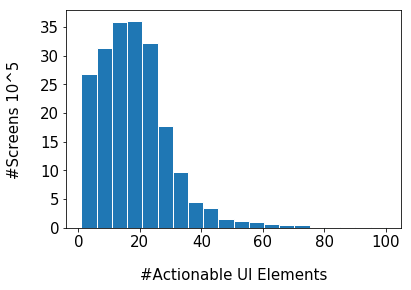
\includegraphics[width=\textwidth]{graphics/zhou_actionable_elements}
    \caption{Number of actionable elements per screen}
    \label{fig:zhou_actionable_elements}
  \end{subfigure}
  \hfill
  \begin{subfigure}[b]{0.3\textwidth}
    \centering
    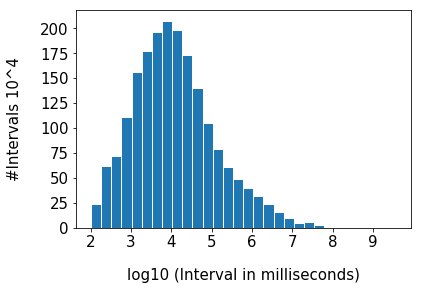
\includegraphics[width=\textwidth]{graphics/zhou_event_time_intervals}
    \caption{The distribution of time intervals between click events}
    \label{fig:zhou_event_time_intervals}
  \end{subfigure}
  \hfill
  \begin{subfigure}[b]{0.3\textwidth}
    \centering
    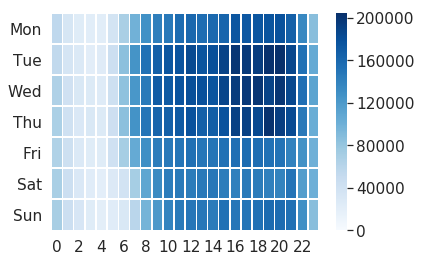
\includegraphics[width=\textwidth]{graphics/zhou_event_time_distribution}
    \caption{The distribution of time intervals between click events}
    \label{fig:zhou_event_time_distribution}
  \end{subfigure}
  \caption[View element insights]{View element insights \cite{zhou2021large}}
  \label{fig:zhou_graphs}
\end{figure}

\todo{provide short summary}
